\documentclass[10pt,a4paper]{article}
\usepackage{tocloft}
\usepackage{commons/course}  % همین کافیه؛ listings و xcolor داخلشه
\usepackage{booktabs}
\usepackage{graphicx}

% Define colors for syntax highlighting
\definecolor{keywordstyle}{rgb}{0.0, 0.4, 0.8}
\definecolor{stringstyle}{rgb}{0.9, 0.17, 0.31}
\definecolor{commentstyle}{rgb}{0.1, 0.6, 0.2}
\definecolor{numberstyle}{rgb}{0.4, 0.4, 0.4}
\definecolor{backgroundcolor}{rgb}{0.94, 0.97, 1.0}

\lstdefinelanguage{ShellLike}{
	morekeywords={PASS,FAIL,Passed,Failed,Running,Loading},
	sensitive=false,
	morecomment=[l]{\#},
	morestring=[b]",
}

\lstset{
	language=ShellLike,
	basicstyle=\ttfamily\scriptsize,
	keywordstyle=\color{keywordstyle}\bfseries,
	stringstyle=\color{stringstyle},
	commentstyle=\color{commentstyle},
	numbers=none,
	keepspaces=true,
	tabsize=2,
	showspaces=false,
	showstringspaces=false,
	showtabs=false,
	breaklines=true,
	breakatwhitespace=false,
	frame=single,
	backgroundcolor=\color{backgroundcolor},
}

\newlistof{listofproblems}{lop}{\normalsize فهرست مسائل}
\newcommand{\addproblem}[1]{\addcontentsline{lop}{listofproblems}{\protect\numberline{}#1}}

\begin{document}

\سربرگ{آزمایش اول}{تشخیص مضرب ۳ و ۱۱ در عدد \lr{BCD}}{}{استاد: دکتر انصاری}

\subsubsection*{خلاصه}

در این آزمایش دو مدار ترکیبی در \lr{Logisim Evolution} پیاده‌سازی شده‌اند که یک عدد \lr{BCD} چهاررقمی را می‌گیرند و مشخص می‌کنند آیا مضرب ۳ (\lr{mod3\_checker}) یا مضرب ۱۱ (\lr{mod11\_checker}) است. فقط از گیت‌های پایه استفاده شده و مدار به‌صورت سلسله‌مراتبی از بلوک‌های \lr{full\_adder}، \lr{adder4}/\lr{adder5} و مقایسه‌گرها ساخته شده است.



\subsubsection*{مضرب ۳ -- جمع ارقام}
چون $10 \equiv 1 \pmod 3$، داریم
\[
N = 1000D_3+100D_2+10D_1+D_0 \;\equiv\; D_3+D_2+D_1+D_0 \pmod 3 .
\]
پس کافی است $S = D_3+D_2+D_1+D_0$ را محاسبه کنیم و ببینیم $S \equiv 0 \pmod 3$ هست یا نه. چون $2 \equiv -1 \pmod 3$، بیت‌های زوج و فرد $S$ وزن $+1$ و $-1$ دارند. با تعریف
\[
P = s_0+s_2+s_4, \qquad Q = s_1+s_3+s_5,
\]
داریم $S \equiv P-Q \pmod 3$. شرط $S \equiv 0$ معادل $P \equiv Q \pmod 3$ است؛ یعنی $P=Q$ یا $\{P,Q\}=\{0,3\}$. خود $P$ و $Q$ با یک \lr{full\_adder} روی سه بیت متناظر به‌دست می‌آیند.

\subsubsection*{مضرب ۱۱ -- جمع متناوب ارقام}
چون $10 \equiv -1 \pmod{11}$:
\[
N \equiv (D_0+D_2)-(D_1+D_3) \pmod{11}.
\]
با $A=D_0+D_2$ و $B=D_1+D_3$، بازه‌ی $A-B$ بین $-18$ تا $+18$ است و تنها مضرب‌های ۱۱ در این بازه $-11$، $0$ و $+11$ هستند. بنابراین
\[
N \equiv 0 \pmod{11} \quad\Longleftrightarrow\quad A+11=B \ \ \text{یا}\ \ A=B \ \ \text{یا}\ \ A=B+11 .
\]
این سه شرط با جمع‌کننده (برای $A+11$ و $B+11$) و مقایسه‌گر تساوی پیاده می‌شوند.

\pagebreak
\subsubsection*{تمام‌جمع‌کننده‌ی ۱ بیتی (\lr{full\_adder})}

\begin{center}
\begin{tabular}{@{}lll@{}}
\toprule
{پایه} & {جهت} & {پهنا} \\
\midrule
\lr{A}, \lr{B}, \lr{Cin} & ورودی & ۱ بیت \\
\lr{S}, \lr{Cout} & خروجی & ۱ بیت \\
\bottomrule
\end{tabular}
\end{center}

مدار با ۲ گیت \lr{XOR}، ۲ گیت \lr{AND} و ۱ گیت \lr{OR} ساخته شده -- بلوک پایه‌ی تمام محاسبات این آزمایش:

\begin{itemize}
    \item $X_1 = A \oplus B$ -- نیمه‌جمع، بدون در نظر گرفتن رقم نقلی ورودی.
    \item $P_1 = A \land B$ -- آیا از جمع $A$ و $B$ به‌تنهایی رقم نقلی تولید می‌شود؟
    \item $S = X_1 \oplus C_{in}$ -- جمع نهایی سه ورودی.
    \item $P_2 = X_1 \land C_{in}$ -- آیا از جمع $X_1$ و $C_{in}$ رقم نقلی تولید می‌شود؟
    \item $C_{out} = P_1 \lor P_2$ -- رقم نقلی خروجی نهایی.
\end{itemize}

\begin{center}
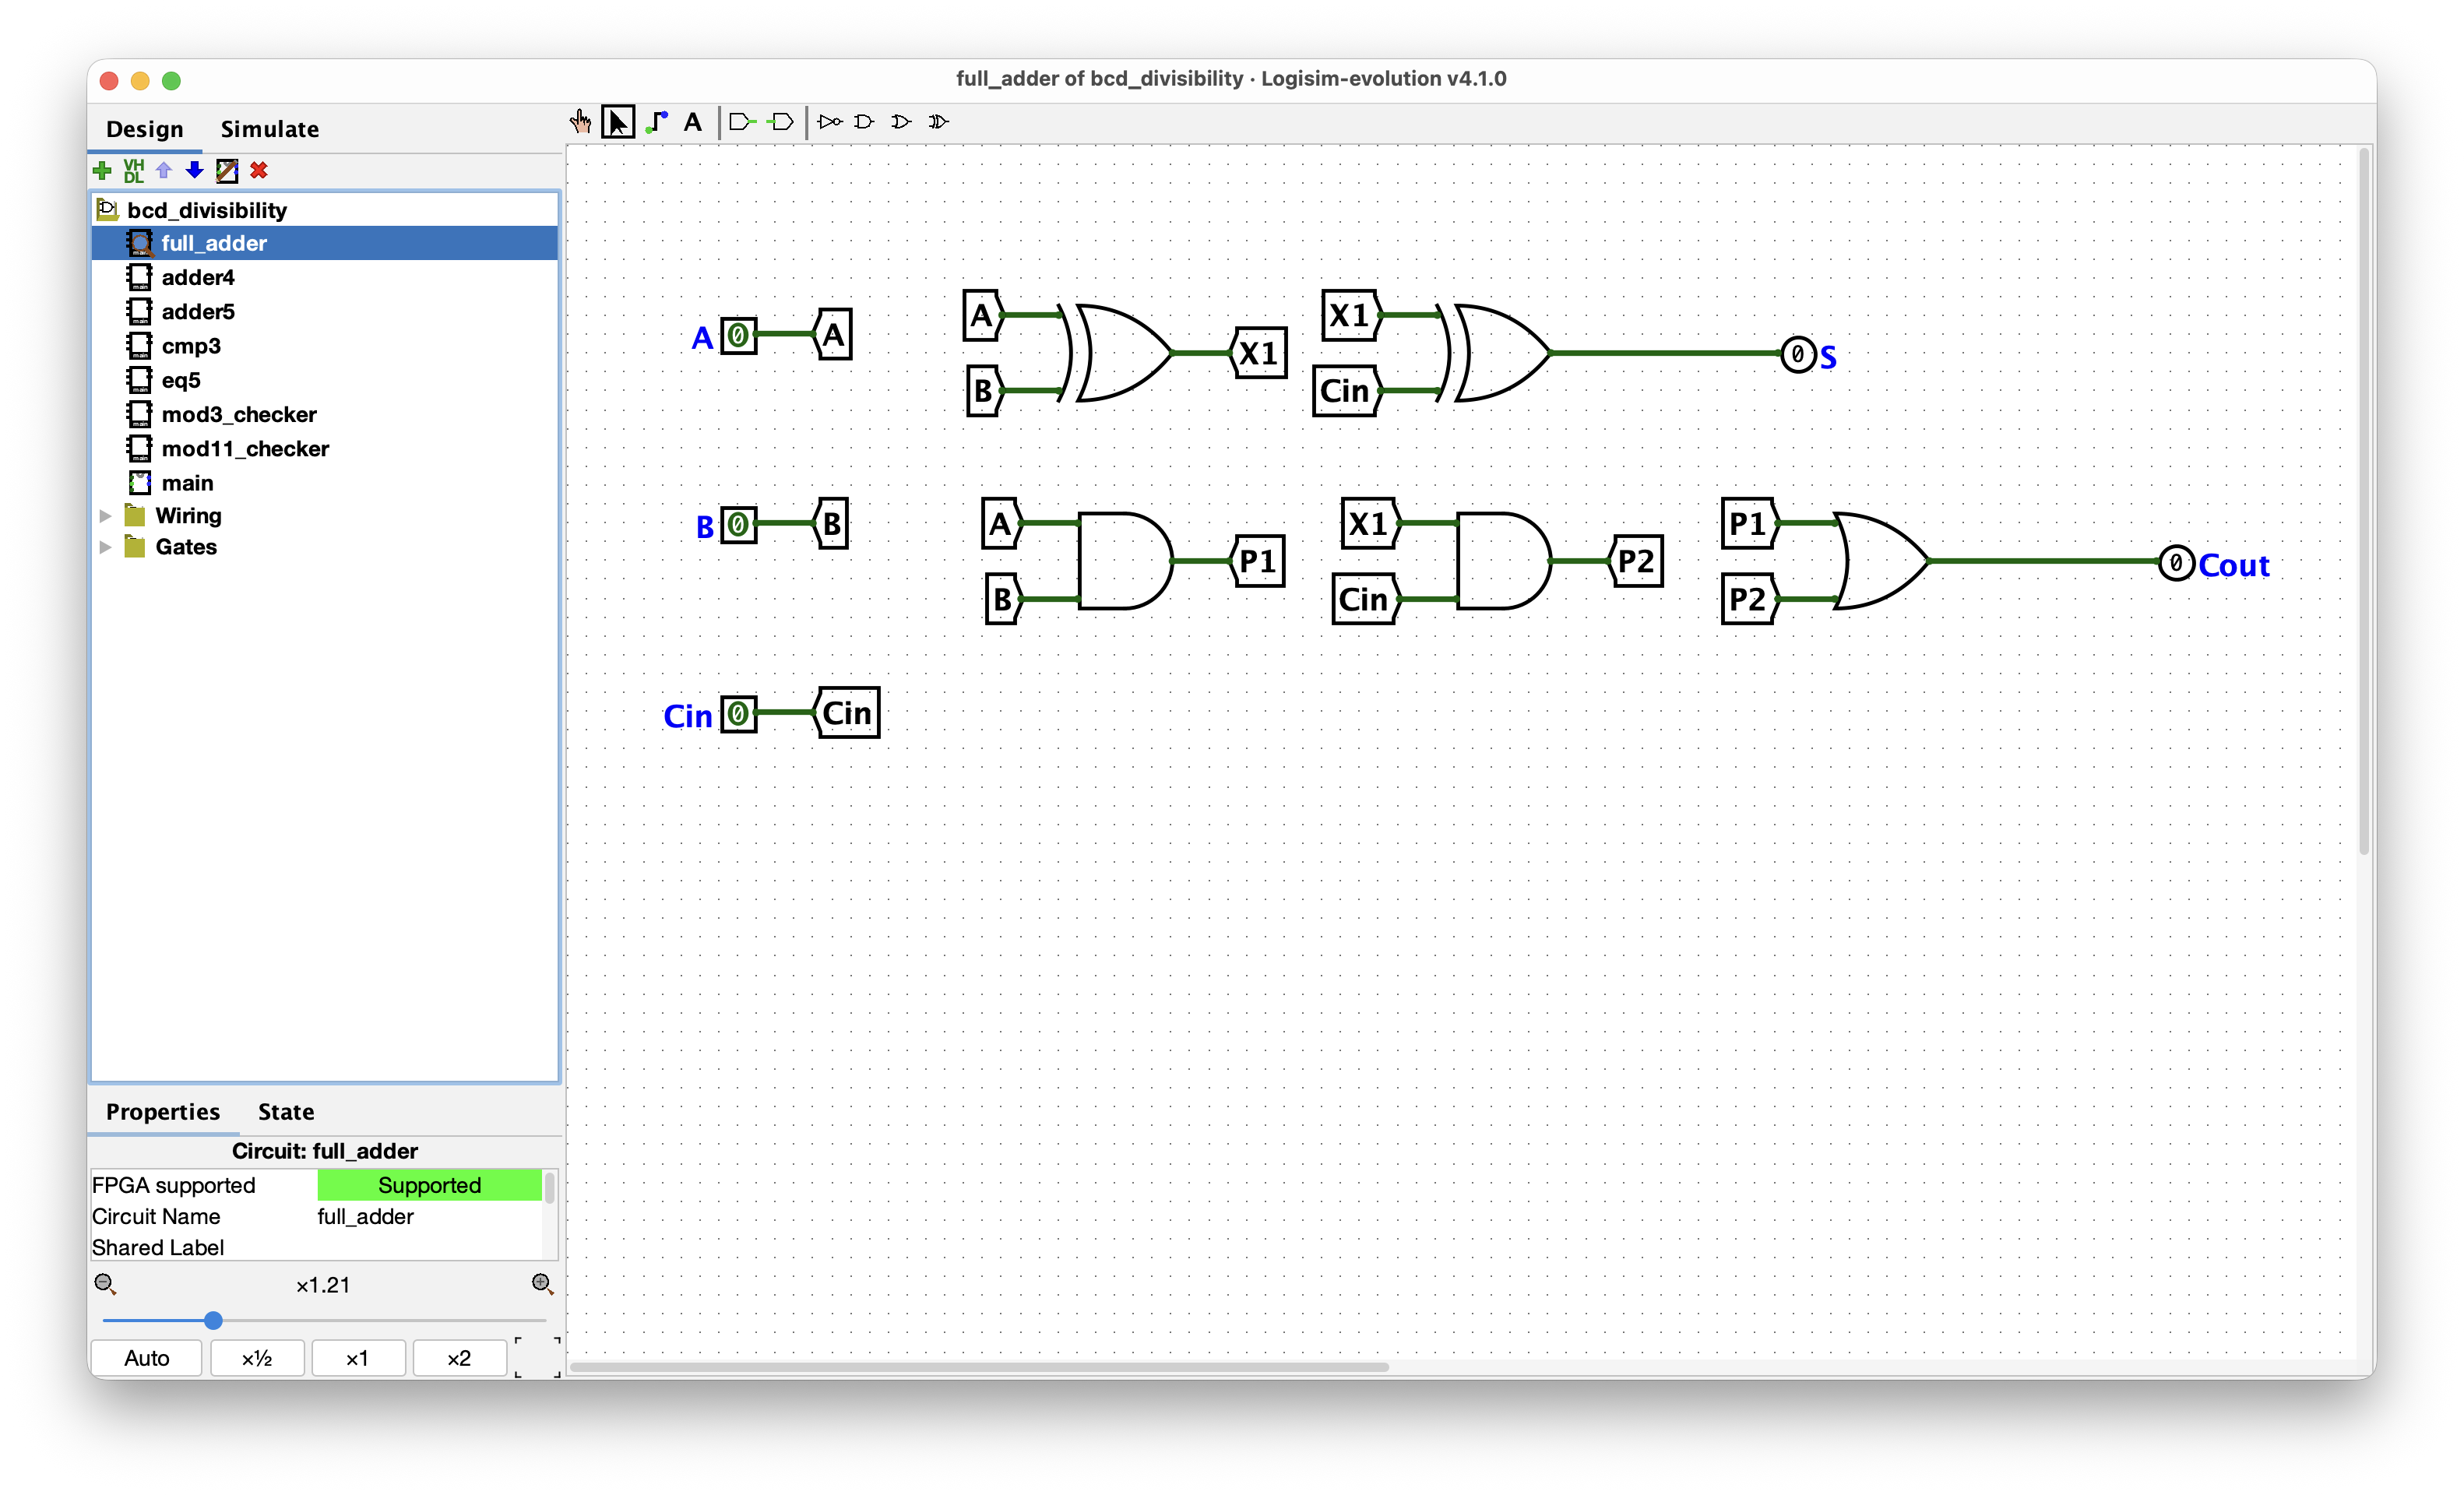
\includegraphics[width=0.85\textwidth]{figs/full-adder.png}
\end{center}

\begin{center}
\begin{latin}
\begin{tabular}{@{}ccc|cc@{}}
\toprule
A & B & Cin & S & Cout \\
\midrule
0 & 0 & 0 & 0 & 0\\
0 & 0 & 1 & 1 & 0\\
0 & 1 & 0 & 1 & 0\\
0 & 1 & 1 & 0 & 1\\
1 & 0 & 0 & 1 & 0\\
1 & 0 & 1 & 0 & 1\\
1 & 1 & 0 & 0 & 1\\
1 & 1 & 1 & 1 & 1\\
\bottomrule
\end{tabular}
\end{latin}
\end{center}

\pagebreak
\subsubsection*{جمع‌کننده‌ی ۴ بیتی (\lr{adder4})}

\begin{center}
\begin{tabular}{@{}lll@{}}
\toprule
{پایه} & {جهت} & {پهنا} \\
\midrule
\lr{A0..A3}, \lr{B0..B3} & ورودی & ۱ بیت هرکدام (جمعا ۸ پایه) \\
\lr{S0..S4} & خروجی & ۱ بیت هرکدام (جمعا ۵ پایه) \\
\bottomrule
\end{tabular}
\end{center}

زنجیره‌ی \lr{ripple-carry} از ۴ نمونه‌ی \lr{full\_adder}: بیت صفر یک نیمه‌جمع‌کننده است (رقم نقلی ورودی‌اش مستقیما به یک قطعه‌ی \lr{Constant} با مقدار \lr{0x0} وصل می‌شود)، و رقم نقلی خروجی هر طبقه به رقم نقلی ورودی طبقه‌ی بعد می‌رود. رقم نقلی خروجی طبقه‌ی آخر همان بیت پرارزش خروجی، $S_4$، است -- چون $9+9=18$ در ۴ بیت جا نمی‌شود، خروجی باید ۵ بیت باشد.

\begin{center}
\begin{latin}
\begin{tabular}{@{}lllll@{}}
\toprule
instance & bit & inputs & sum out & carry out \\
\midrule
FA0 & 0 (LSB) & $A_0,B_0,\text{GND}$ & $S_0$ & $C_1$ \\
FA1 & 1 & $A_1,B_1,C_1$ & $S_1$ & $C_2$ \\
FA2 & 2 & $A_2,B_2,C_2$ & $S_2$ & $C_3$ \\
FA3 & 3 (MSB) & $A_3,B_3,C_3$ & $S_3$ & $S_4$ \\
\bottomrule
\end{tabular}
\end{latin}
\end{center}

\begin{center}
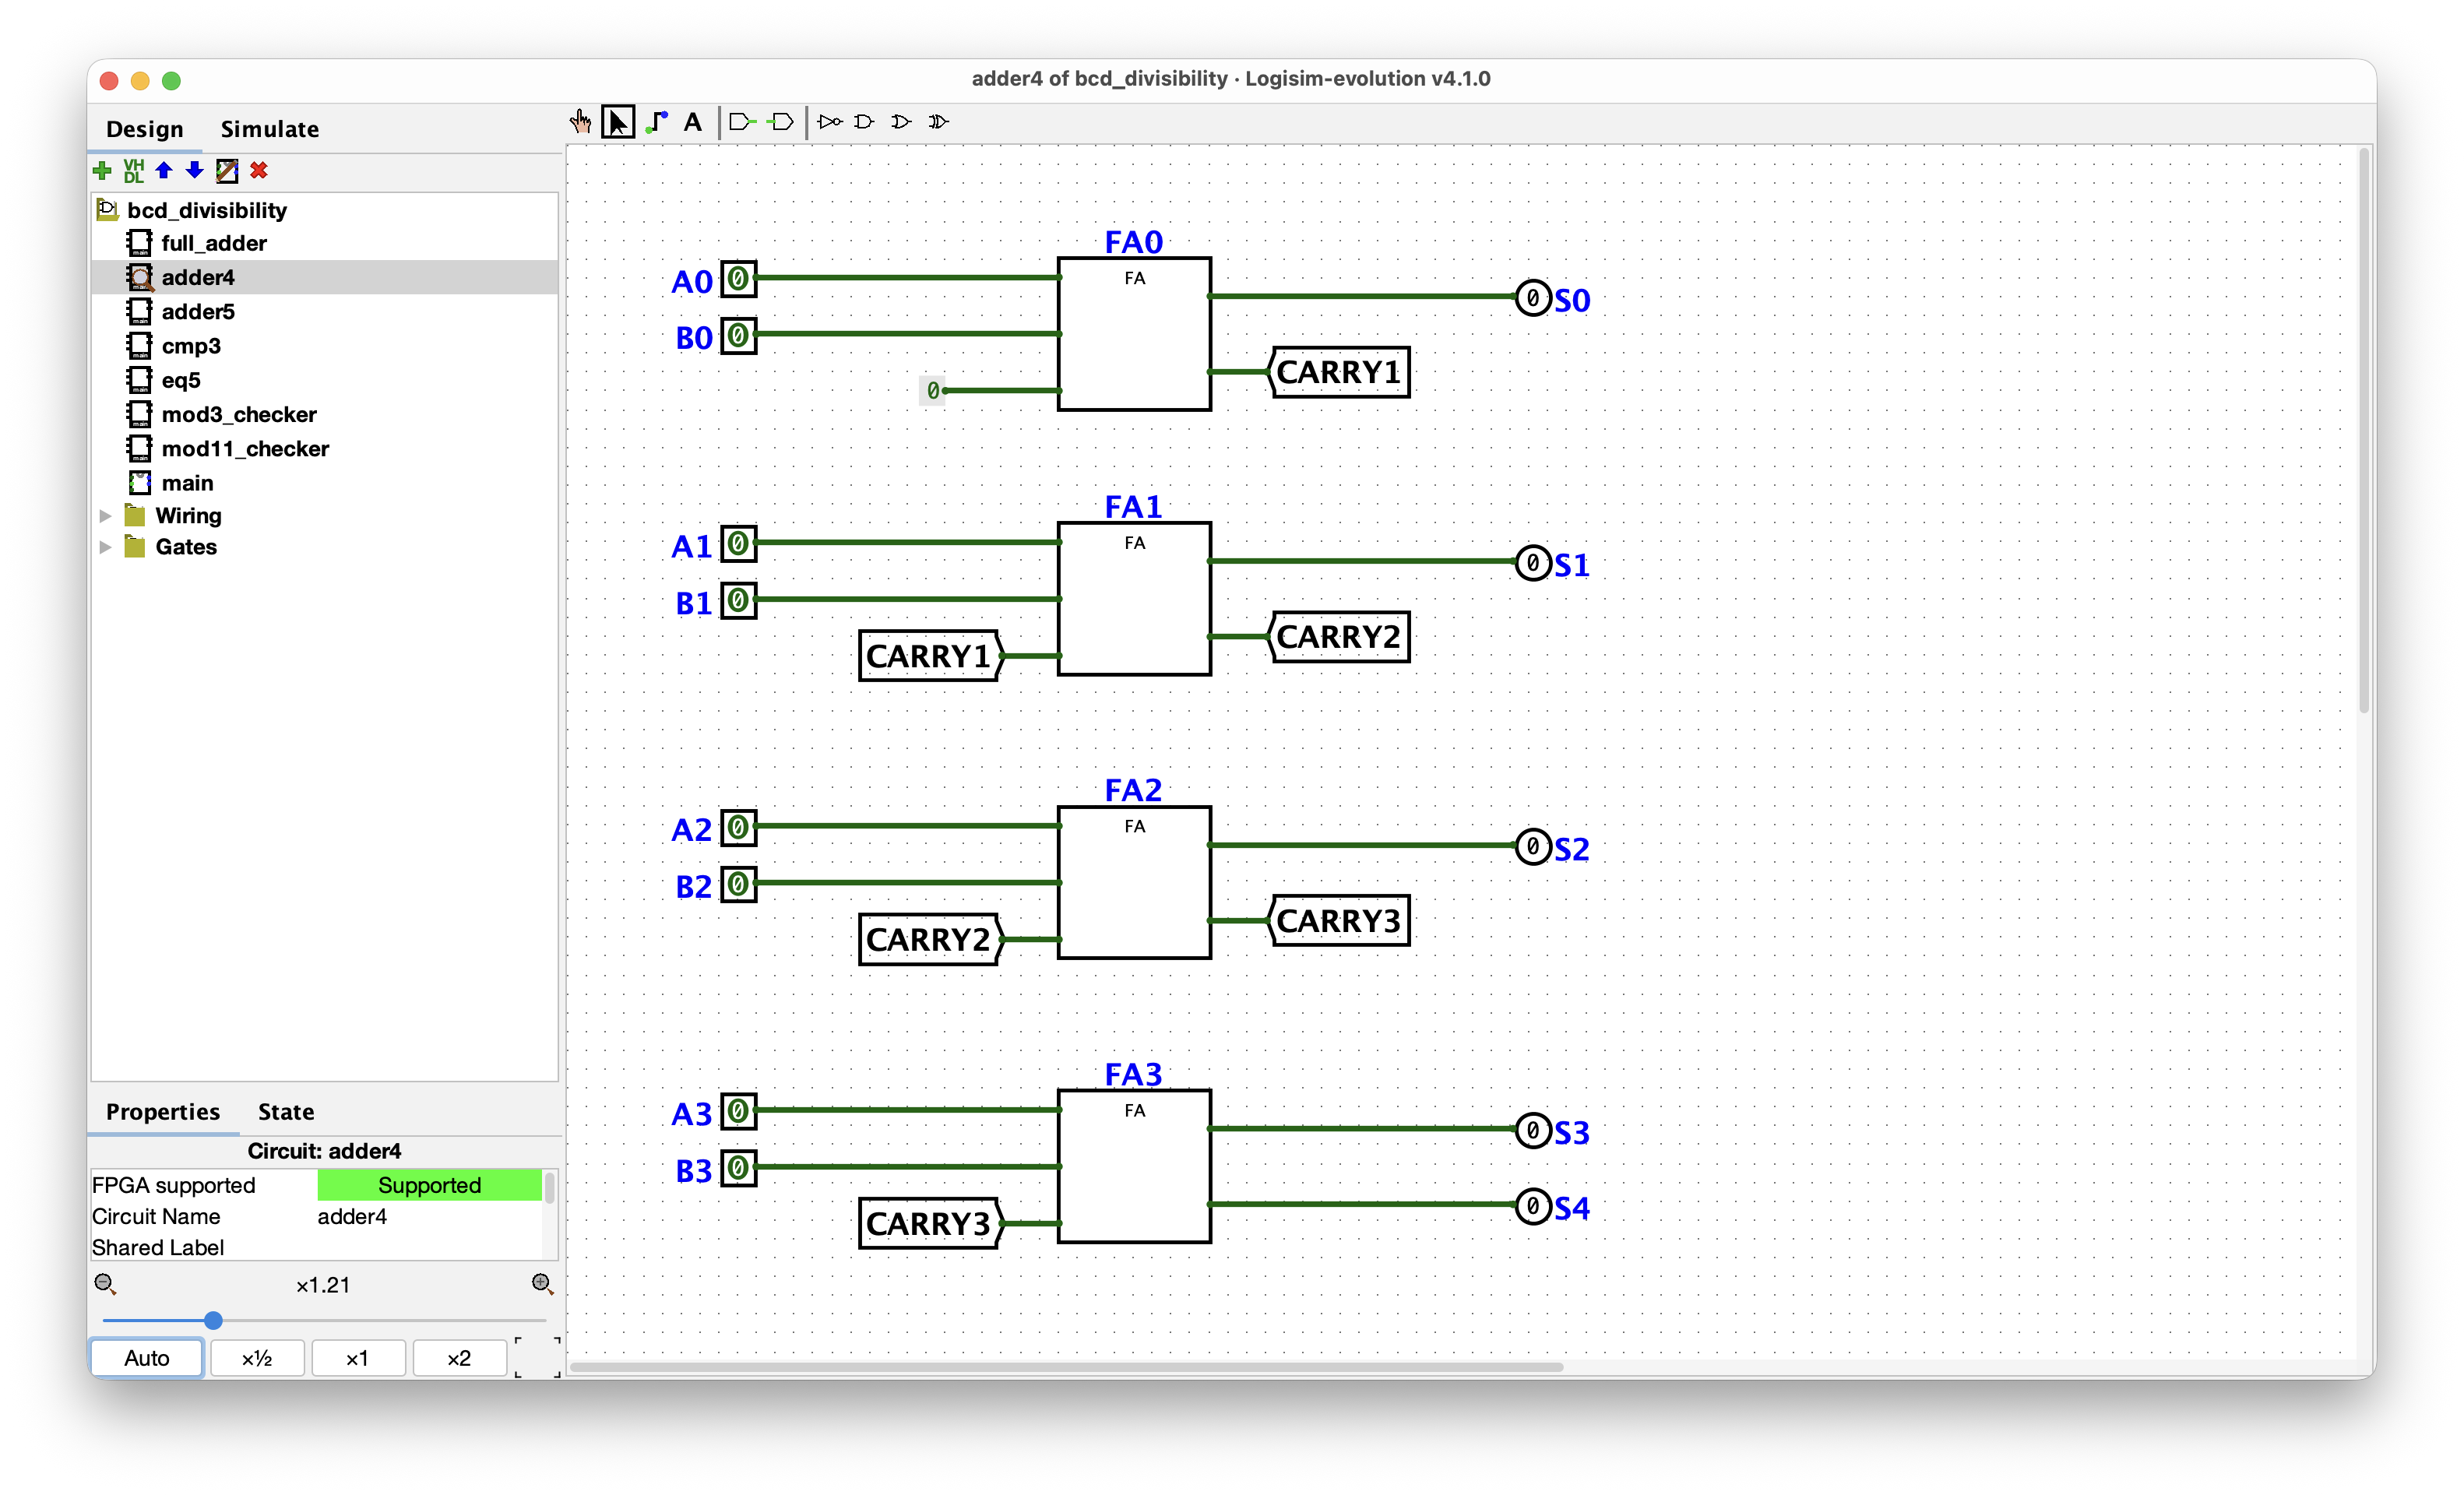
\includegraphics[width=0.9\textwidth]{figs/adder4.png}
\end{center}

\pagebreak

\subsubsection*{جمع‌کننده‌ی ۵ بیتی (\lr{adder5})}

\begin{center}
\begin{tabular}{@{}lll@{}}
\toprule
{پایه} & {جهت} & {پهنا} \\
\midrule
\lr{A0..A4}, \lr{B0..B4} & ورودی & ۱ بیت هرکدام (جمعا ۱۰ پایه) \\
\lr{S0..S5} & خروجی & ۱ بیت هرکدام (جمعا ۶ پایه) \\
\bottomrule
\end{tabular}
\end{center}

دقیقا همان الگوی \lr{adder4}، فقط با ۵ نمونه‌ی \lr{full\_adder} به‌جای ۴ (رقم نقلی ورودی طبقه‌ی صفر باز هم به \lr{GND}). دو کاربرد در این آزمایش: در \lr{mod3\_checker} برای جمع نهایی دو مجموع ۵بیتی $S_{ab}$ و $S_{cd}$ به یک عدد ۶بیتی، و در \lr{mod11\_checker} برای جمع یک عدد ۵بیتی با ثابت ۱۱ (\lr{AP11}, \lr{BP11}).

\begin{center}
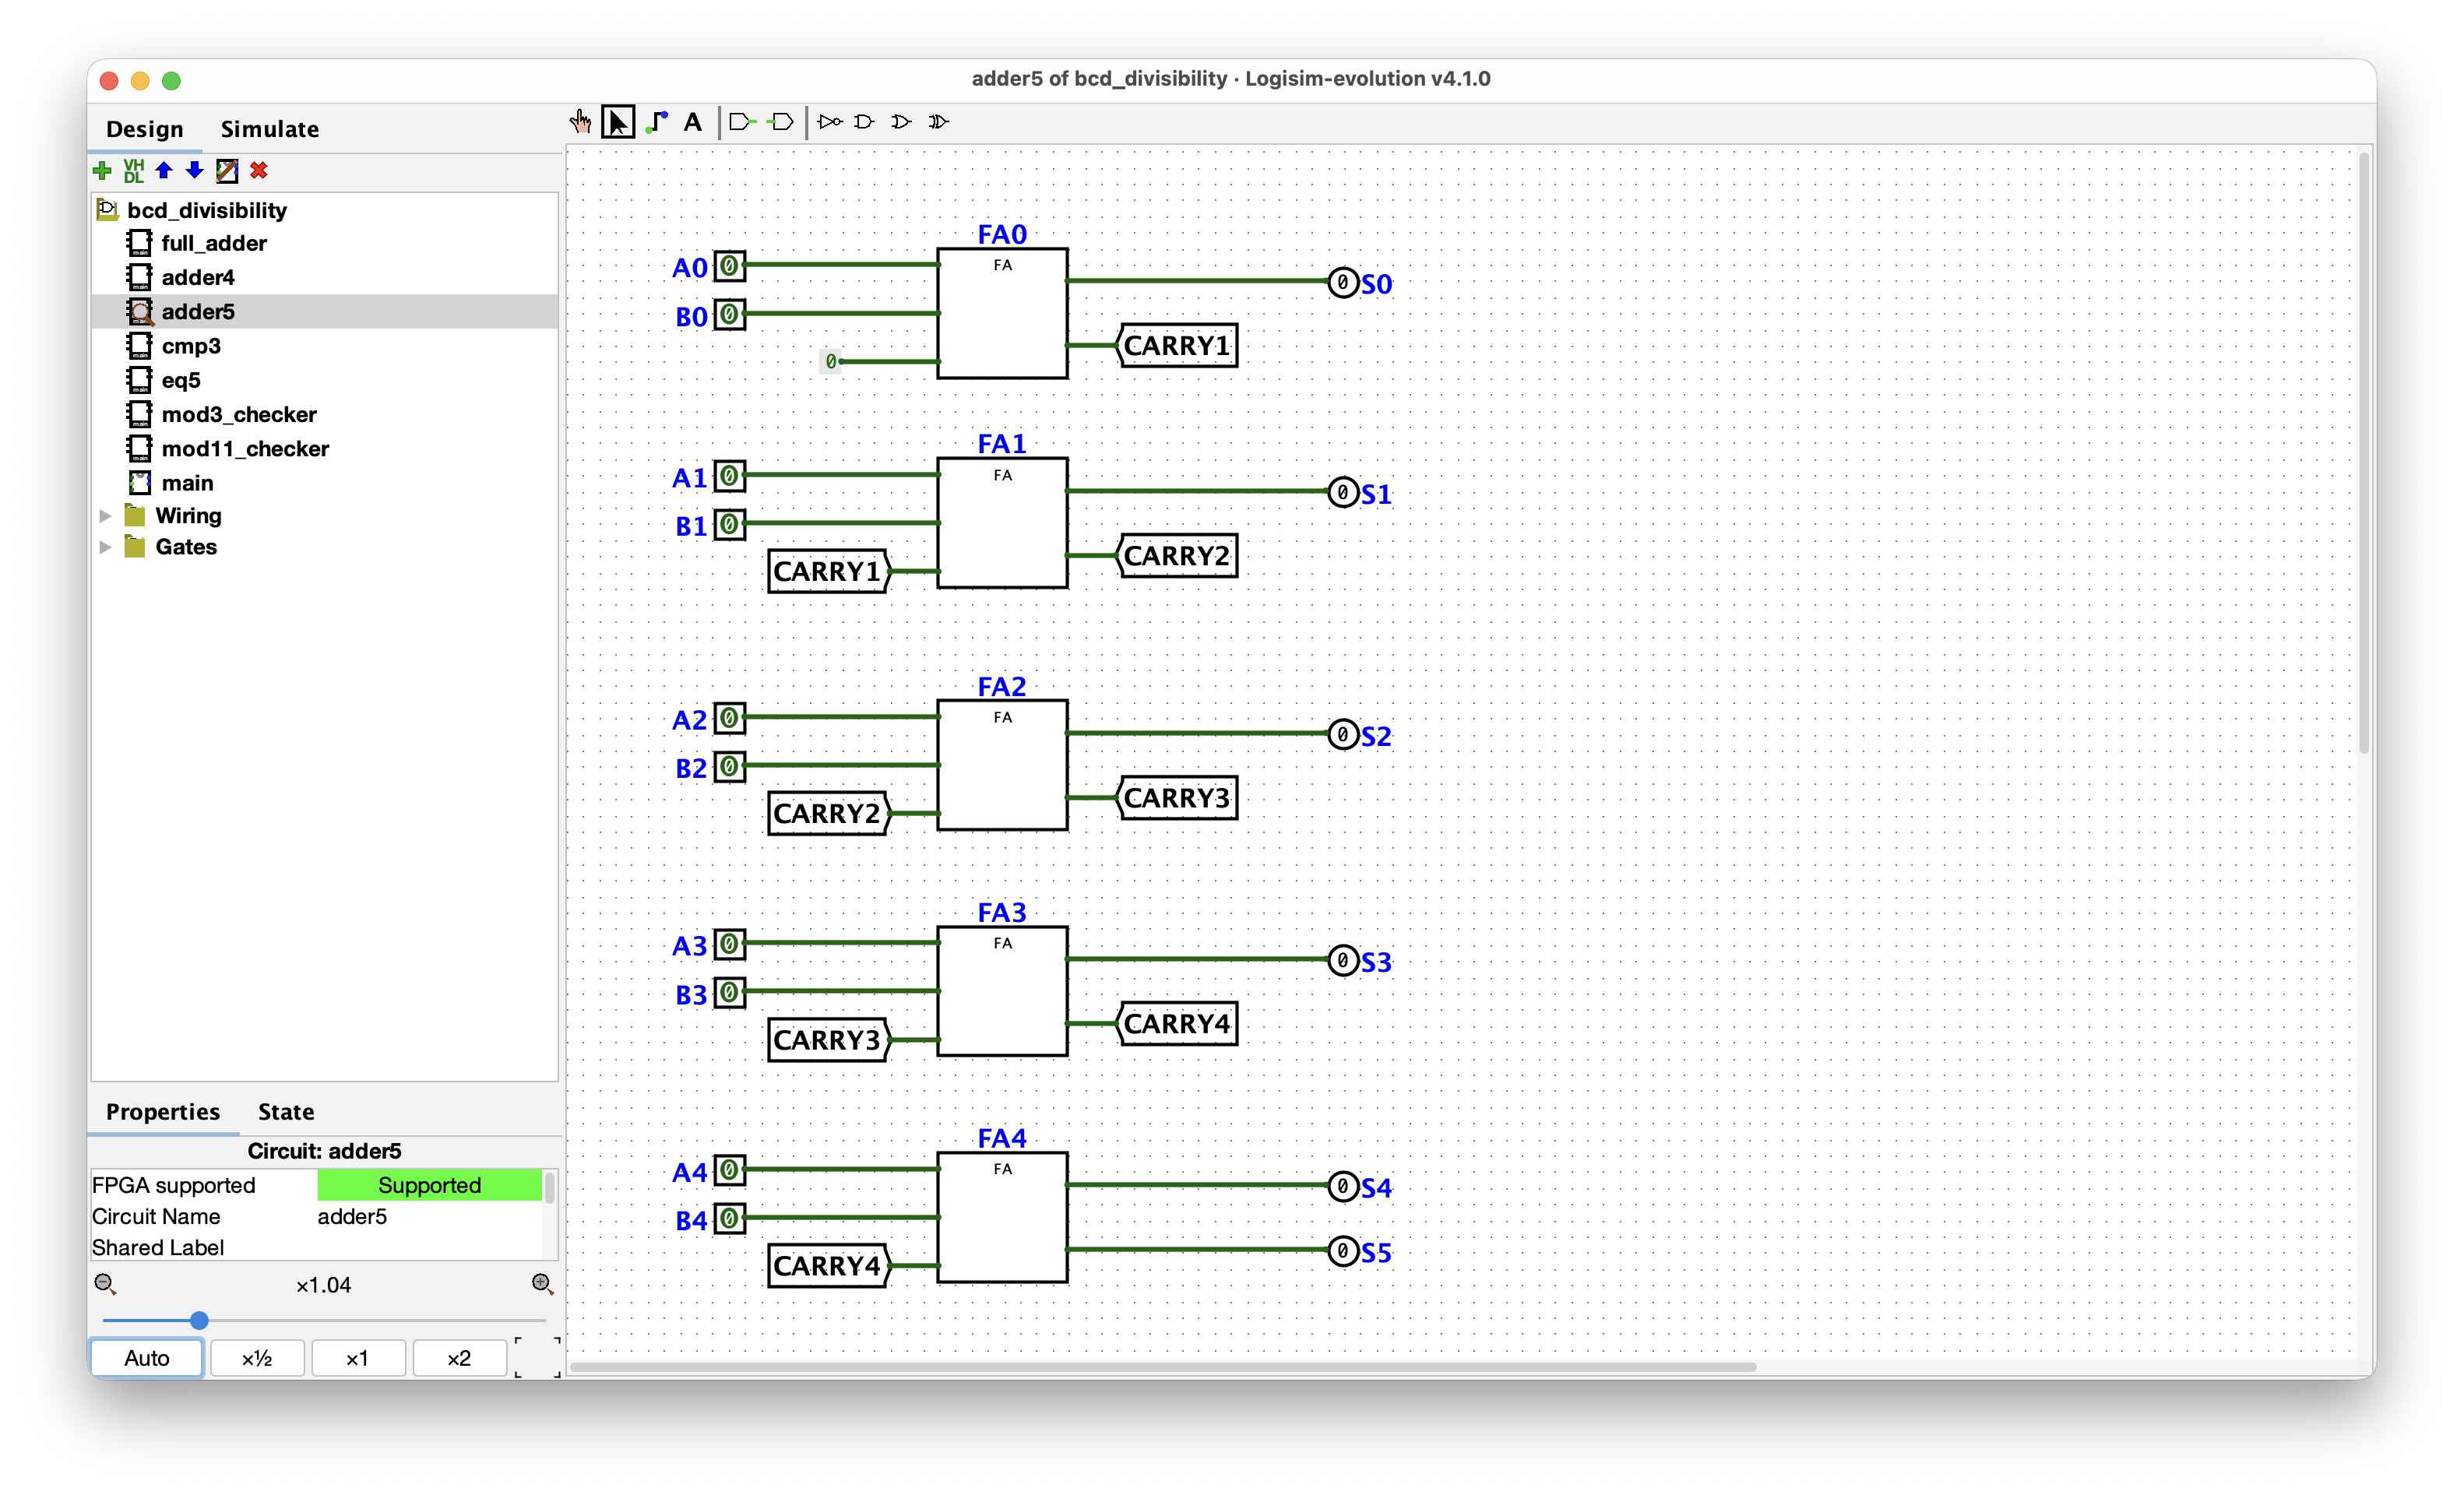
\includegraphics[width=0.9\textwidth]{figs/adder5.png}
\end{center}

\pagebreak

\subsubsection*{مقایسه‌گر \lr{mod} ۳ (\lr{cmp3})}

\begin{center}
\begin{tabular}{@{}lll@{}}
\toprule
{پایه} & {جهت} & {پهنا} \\
\midrule
\lr{p1}, \lr{p0}, \lr{q1}, \lr{q0} & ورودی & ۱ بیت هرکدام \\
\lr{Eq} & خروجی & ۱ بیت \\
\bottomrule
\end{tabular}
\end{center}

شرط $P \bmod 3 = Q \bmod 3$ را برای $P,Q \in \{0,1,2,3\}$ (بیت‌های \lr{p1p0} و \lr{q1q0}) چک می‌کند -- یعنی یا $P{=}Q$، یا $\{P,Q\}{=}\{0,3\}$ (چون $3 \equiv 0 \pmod 3$). نام‌گذاری سیگنال‌های زیر عینا همان نام تونل‌هایی است که در مدار (\lr{cmp3} داخل \lr{bcd\_divisibility.circ}) استفاده شده:

\begin{itemize}
  \item $\mathrm{XORHI} = p_1 \oplus q_1$، $\mathrm{XORLO} = p_0 \oplus q_0$ -- دو \lr{XOR} خام.
  \item $\mathrm{NP}_1 = \overline{p_1}$، $\mathrm{NP}_0 = \overline{p_0}$، $\mathrm{NQ}_1 = \overline{q_1}$، $\mathrm{NQ}_0 = \overline{q_0}$ -- چهار \lr{NOT} خام.
  \item $\mathrm{EQHI} = \overline{\mathrm{XORHI}}$ -- آیا $p_1{=}q_1$؟ \quad $\mathrm{EQLO} = \overline{\mathrm{XORLO}}$ -- آیا $p_0{=}q_0$؟ (این دو با هم، \lr{XNOR} روی گیت‌های پایه‌اند: \lr{XOR}+\lr{NOT}.)
  \item $\mathrm{A}_{0\mathrm{T}} = \mathrm{NP}_1\land\mathrm{NP}_0$ -- شرط $P{=}0$. \quad $\mathrm{B}_{0\mathrm{T}} = q_1\land q_0$ -- شرط $Q{=}3$.
  \item $\mathrm{C}_{0\mathrm{T}} = p_1\land p_0$ -- شرط $P{=}3$. \quad $\mathrm{D}_{0\mathrm{T}} = \mathrm{NQ}_1\land\mathrm{NQ}_0$ -- شرط $Q{=}0$.
  \item $T_1 = \mathrm{EQHI}\land\mathrm{EQLO}$ -- شرط $P{=}Q$.
  \item $T_2 = \mathrm{A}_{0\mathrm{T}}\land\mathrm{B}_{0\mathrm{T}}$ -- شرط $P{=}0 \land Q{=}3$. \quad $T_3 = \mathrm{C}_{0\mathrm{T}}\land\mathrm{D}_{0\mathrm{T}}$ -- شرط $P{=}3 \land Q{=}0$.
  \item $\mathrm{OR}_1 = T_1\lor T_2$، و در نهایت $\mathrm{Eq} = \mathrm{OR}_1\lor T_3$.
\end{itemize}

\begin{center}
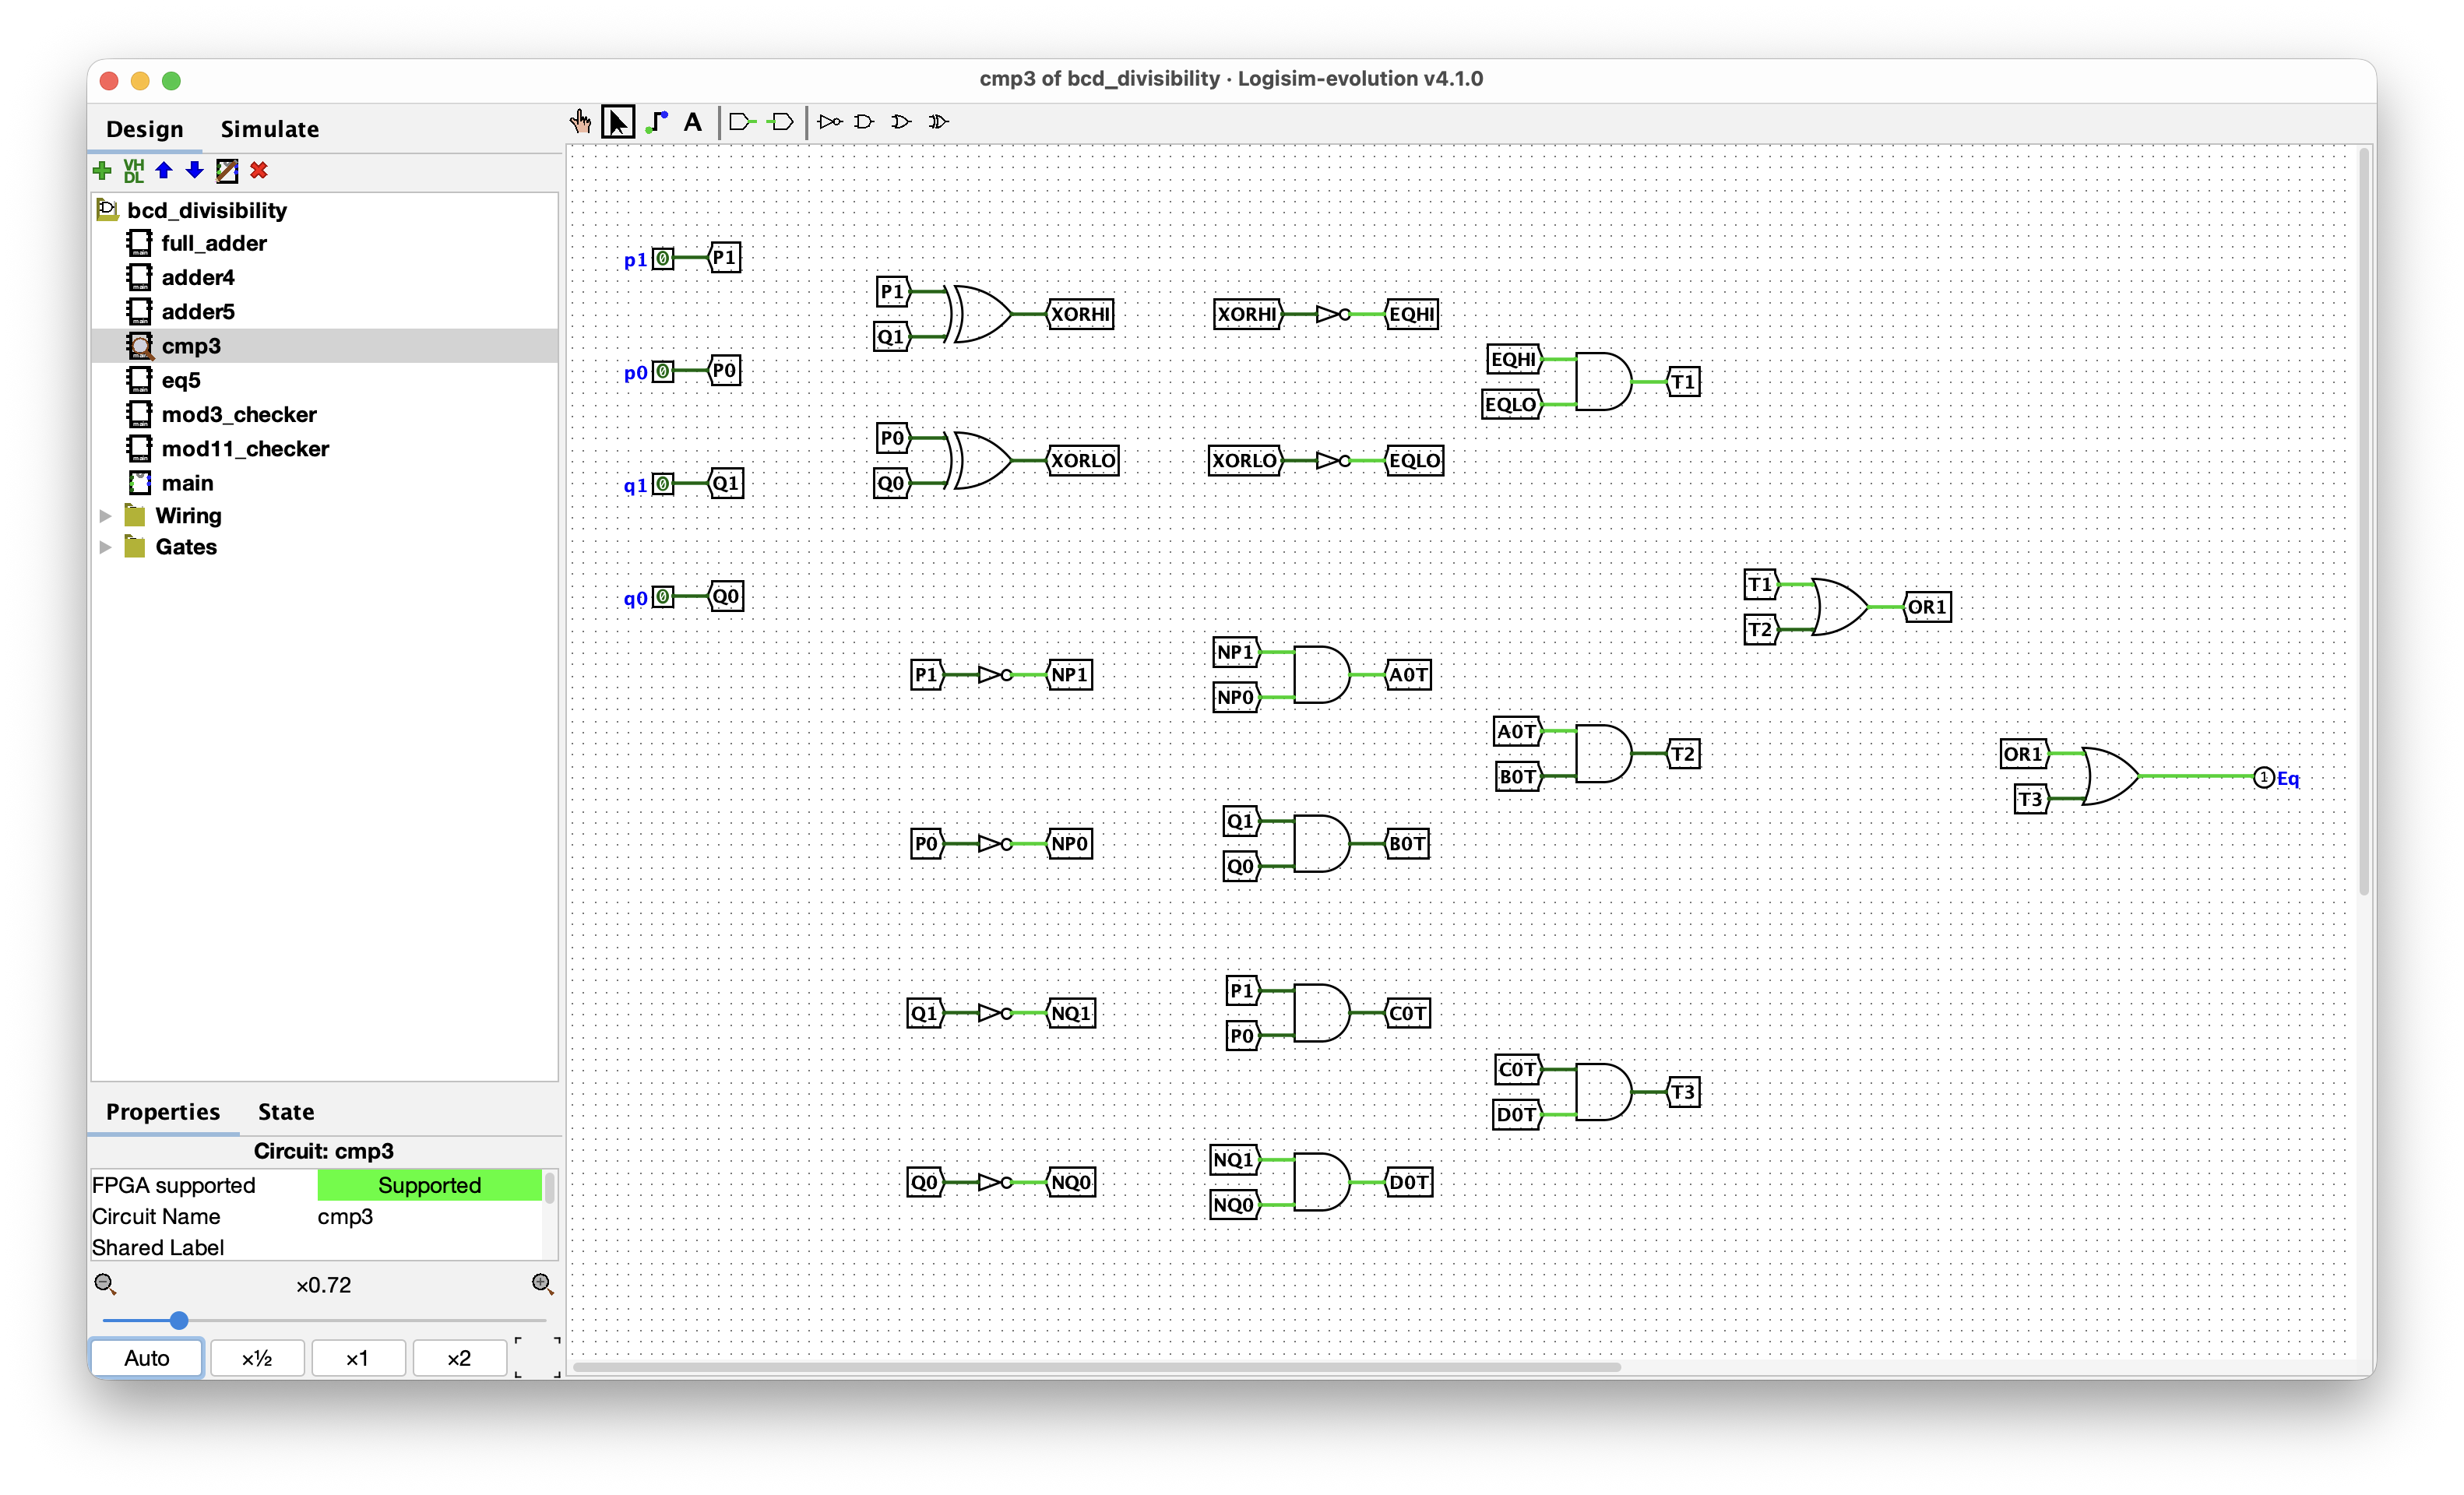
\includegraphics[width=0.85\textwidth]{figs/cmp3.png}
\end{center}

\begin{center}
\begin{latin}
\begin{tabular}{@{}cccc|c@{}}
\toprule
p1 & p0 & q1 & q0 & Eq \\
\midrule
0&0&0&0&1\\
0&0&0&1&0\\
0&0&1&0&0\\
0&0&1&1&1\\
0&1&0&0&0\\
0&1&0&1&1\\
0&1&1&0&0\\
0&1&1&1&0\\
1&0&0&0&0\\
1&0&0&1&0\\
1&0&1&0&1\\
1&0&1&1&0\\
1&1&0&0&1\\
1&1&0&1&0\\
1&1&1&0&0\\
1&1&1&1&1\\
\bottomrule
\end{tabular}
\end{latin}
\end{center}


\subsubsection*{مقایسه‌گر تساوی ۵ بیتی (\lr{eq5})}

\begin{center}
\begin{tabular}{@{}lll@{}}
\toprule
{پایه} & {جهت} & {پهنا} \\
\midrule
\lr{A0..A4}, \lr{B0..B4} & ورودی & ۱ بیت هرکدام (جمعا ۱۰ پایه) \\
\lr{Eq} & خروجی & ۱ بیت \\
\bottomrule
\end{tabular}
\end{center}

بررسی می‌کند آیا دو عدد ۵بیتی $A$ و $B$ برابرند. نام‌گذاری زیر عینا همان نام تونل‌های مدار \lr{eq5} است: برای هر بیت $i$ (۰ تا ۴) یک گیت \lr{XOR} خام $X_i = A_i \oplus B_i$ ساخته می‌شود و بعد یک \lr{NOT} روی آن، $N_i = \overline{X_i}$ (یعنی \lr{XNOR} با گیت‌های پایه) -- که ۱ است دقیقا وقتی $A_i{=}B_i$. سپس پنج نتیجه با یک درخت \lr{AND} ترکیب می‌شوند:
\[
\mathrm{Eq} = N_0 \land N_1 \land N_2 \land N_3 \land N_4 .
\]
درخت به‌صورت متوازن ساخته شده تا عمق مسیر ترکیبی کم بماند -- دقیقا با همین نام‌های تونل در مدار: $\mathrm{T1} = N_0{\land}N_1$، $\mathrm{T2} = N_2{\land}N_3$، $\mathrm{T3} = \mathrm{T1}\land\mathrm{T2}$، و در نهایت $\mathrm{Eq} = \mathrm{T3}\land N_4$. در این آزمایش سه نمونه از \lr{eq5} در \lr{mod11\_checker} استفاده شده‌اند: $AP11{=}B$، $A{=}B$ و $A{=}BP11$.

\begin{center}
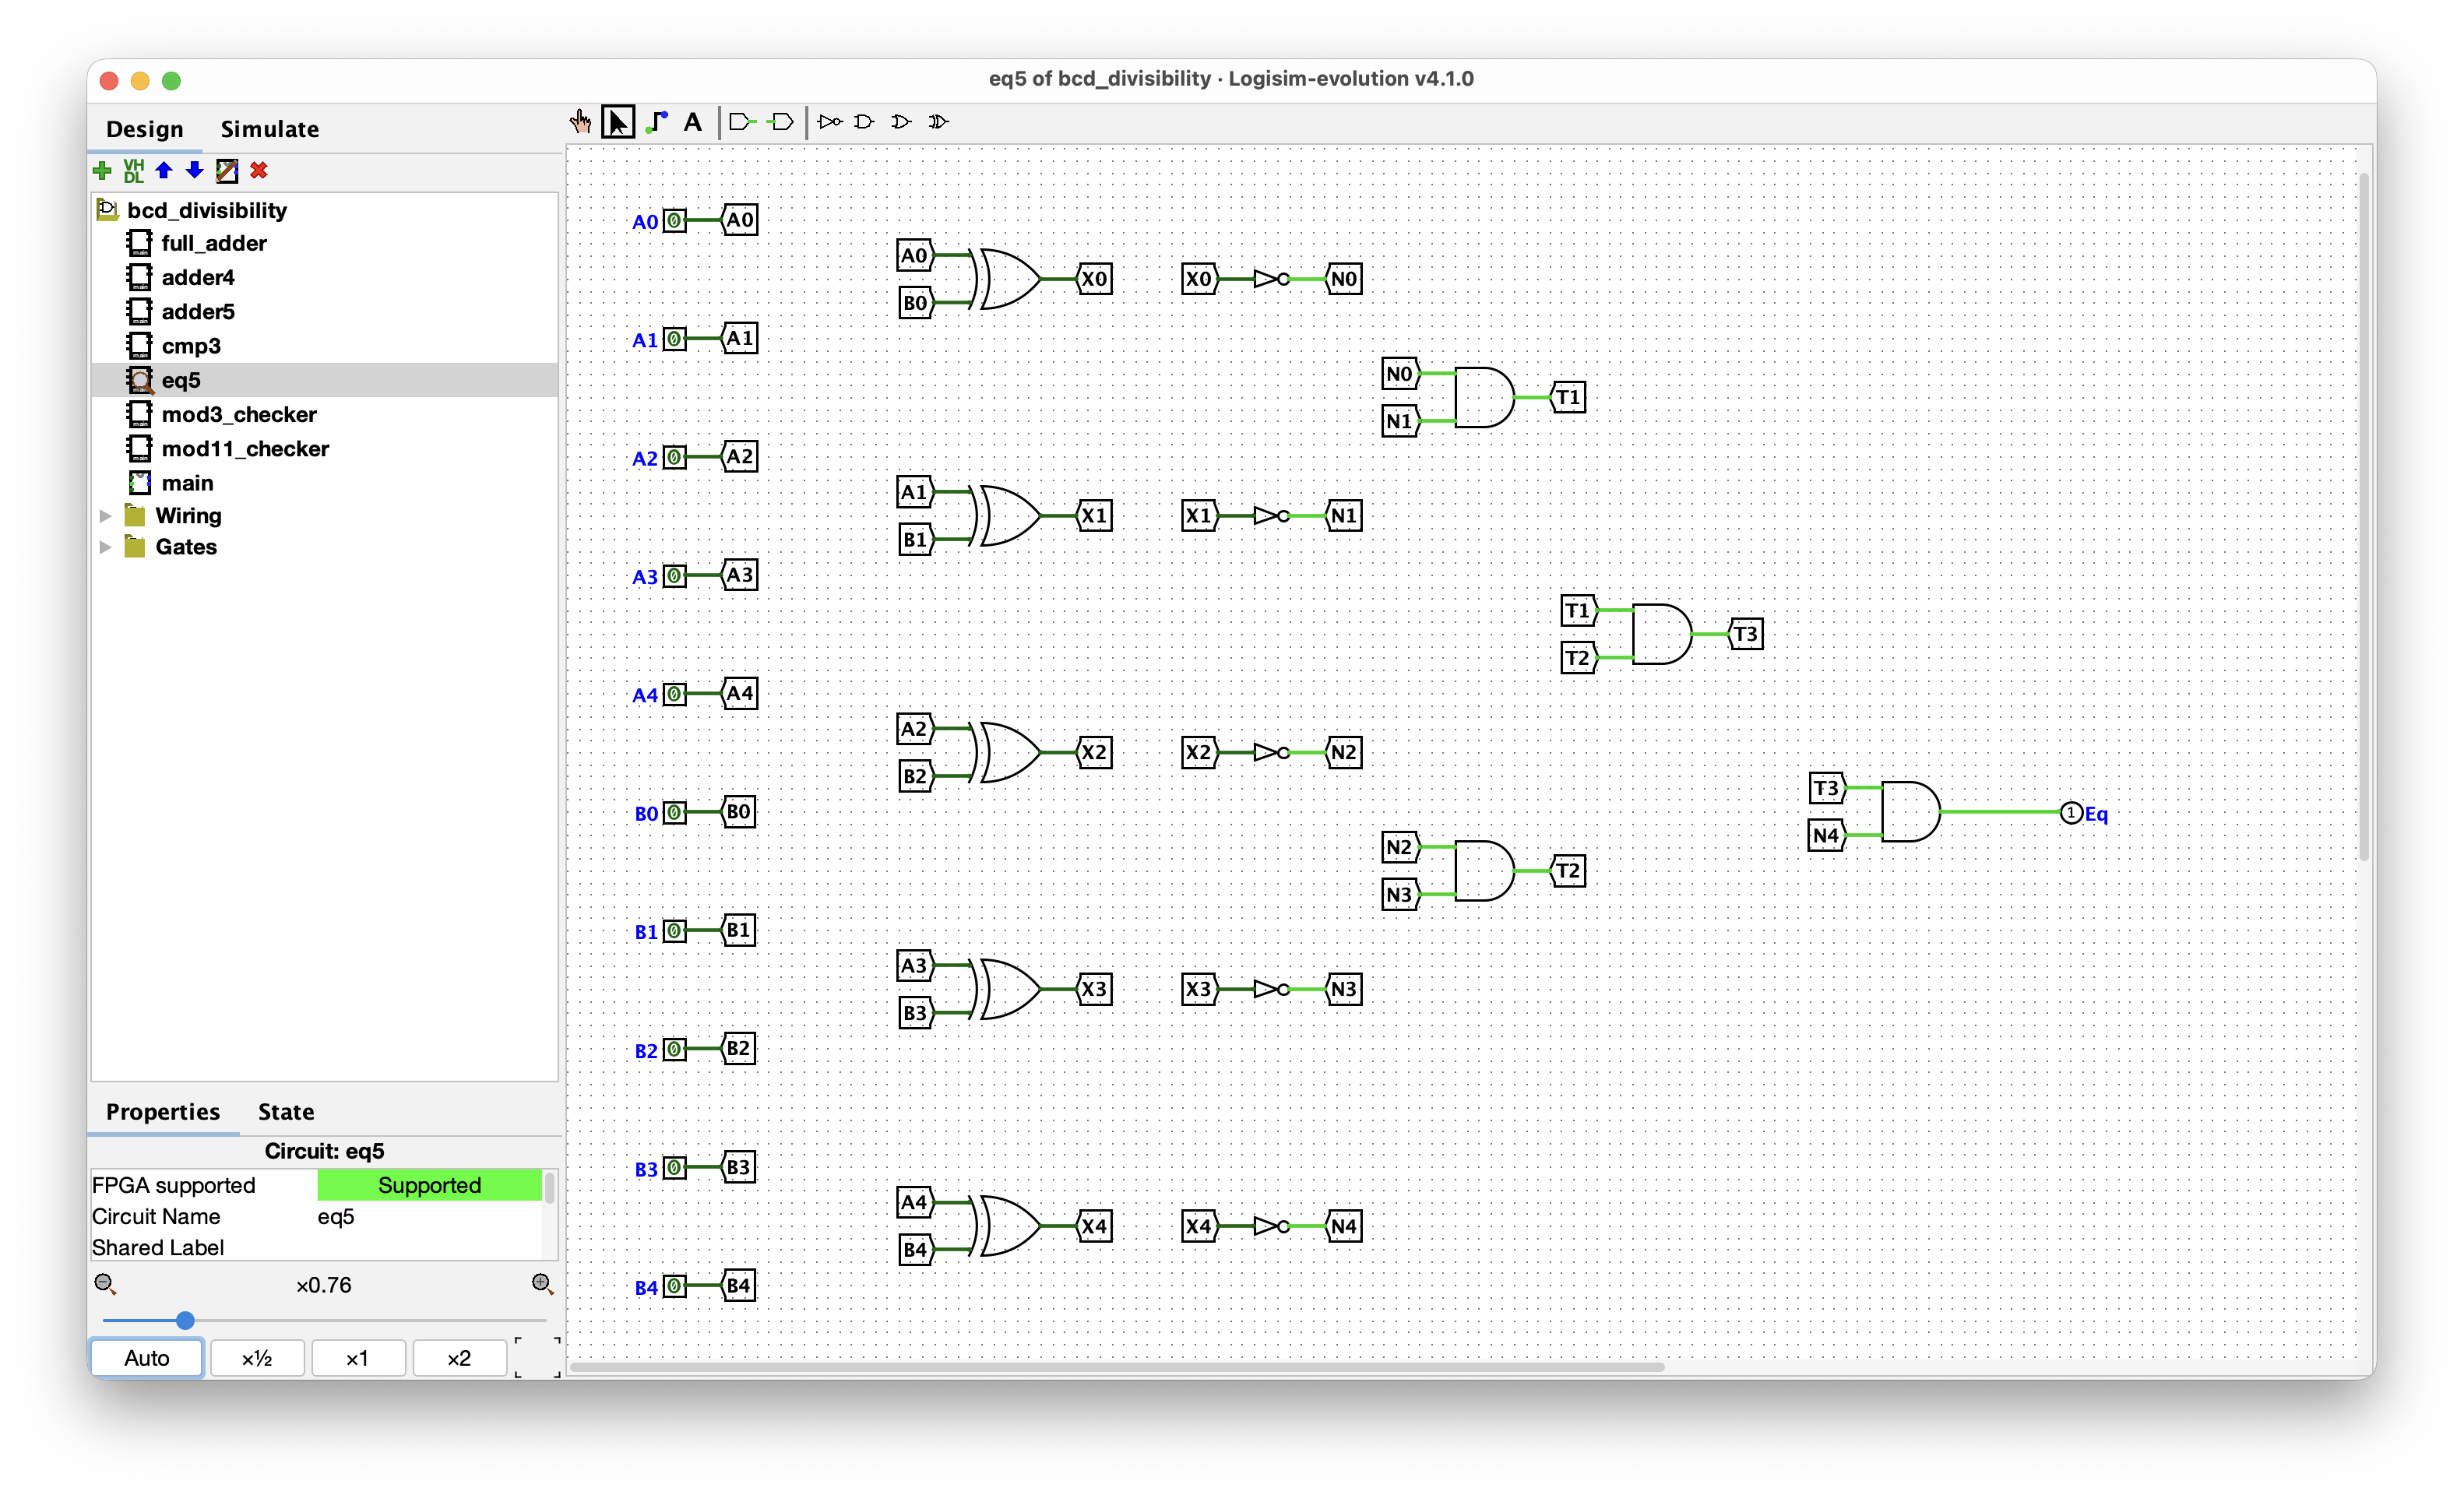
\includegraphics[width=0.9\textwidth]{figs/eq5.png}
\end{center}


\subsubsection*{معماری \lr{mod3\_checker}}

\begin{center}
\begin{tabular}{@{}lll@{}}
\toprule
{پایه} & {جهت} & {پهنا} \\
\midrule
\lr{D0}, \lr{D1}, \lr{D2}, \lr{D3} & ورودی & ۴ بیت (رقم \lr{BCD}) \\
\lr{out} & خروجی & ۱ بیت \\
\bottomrule
\end{tabular}
\end{center}

\begin{center}
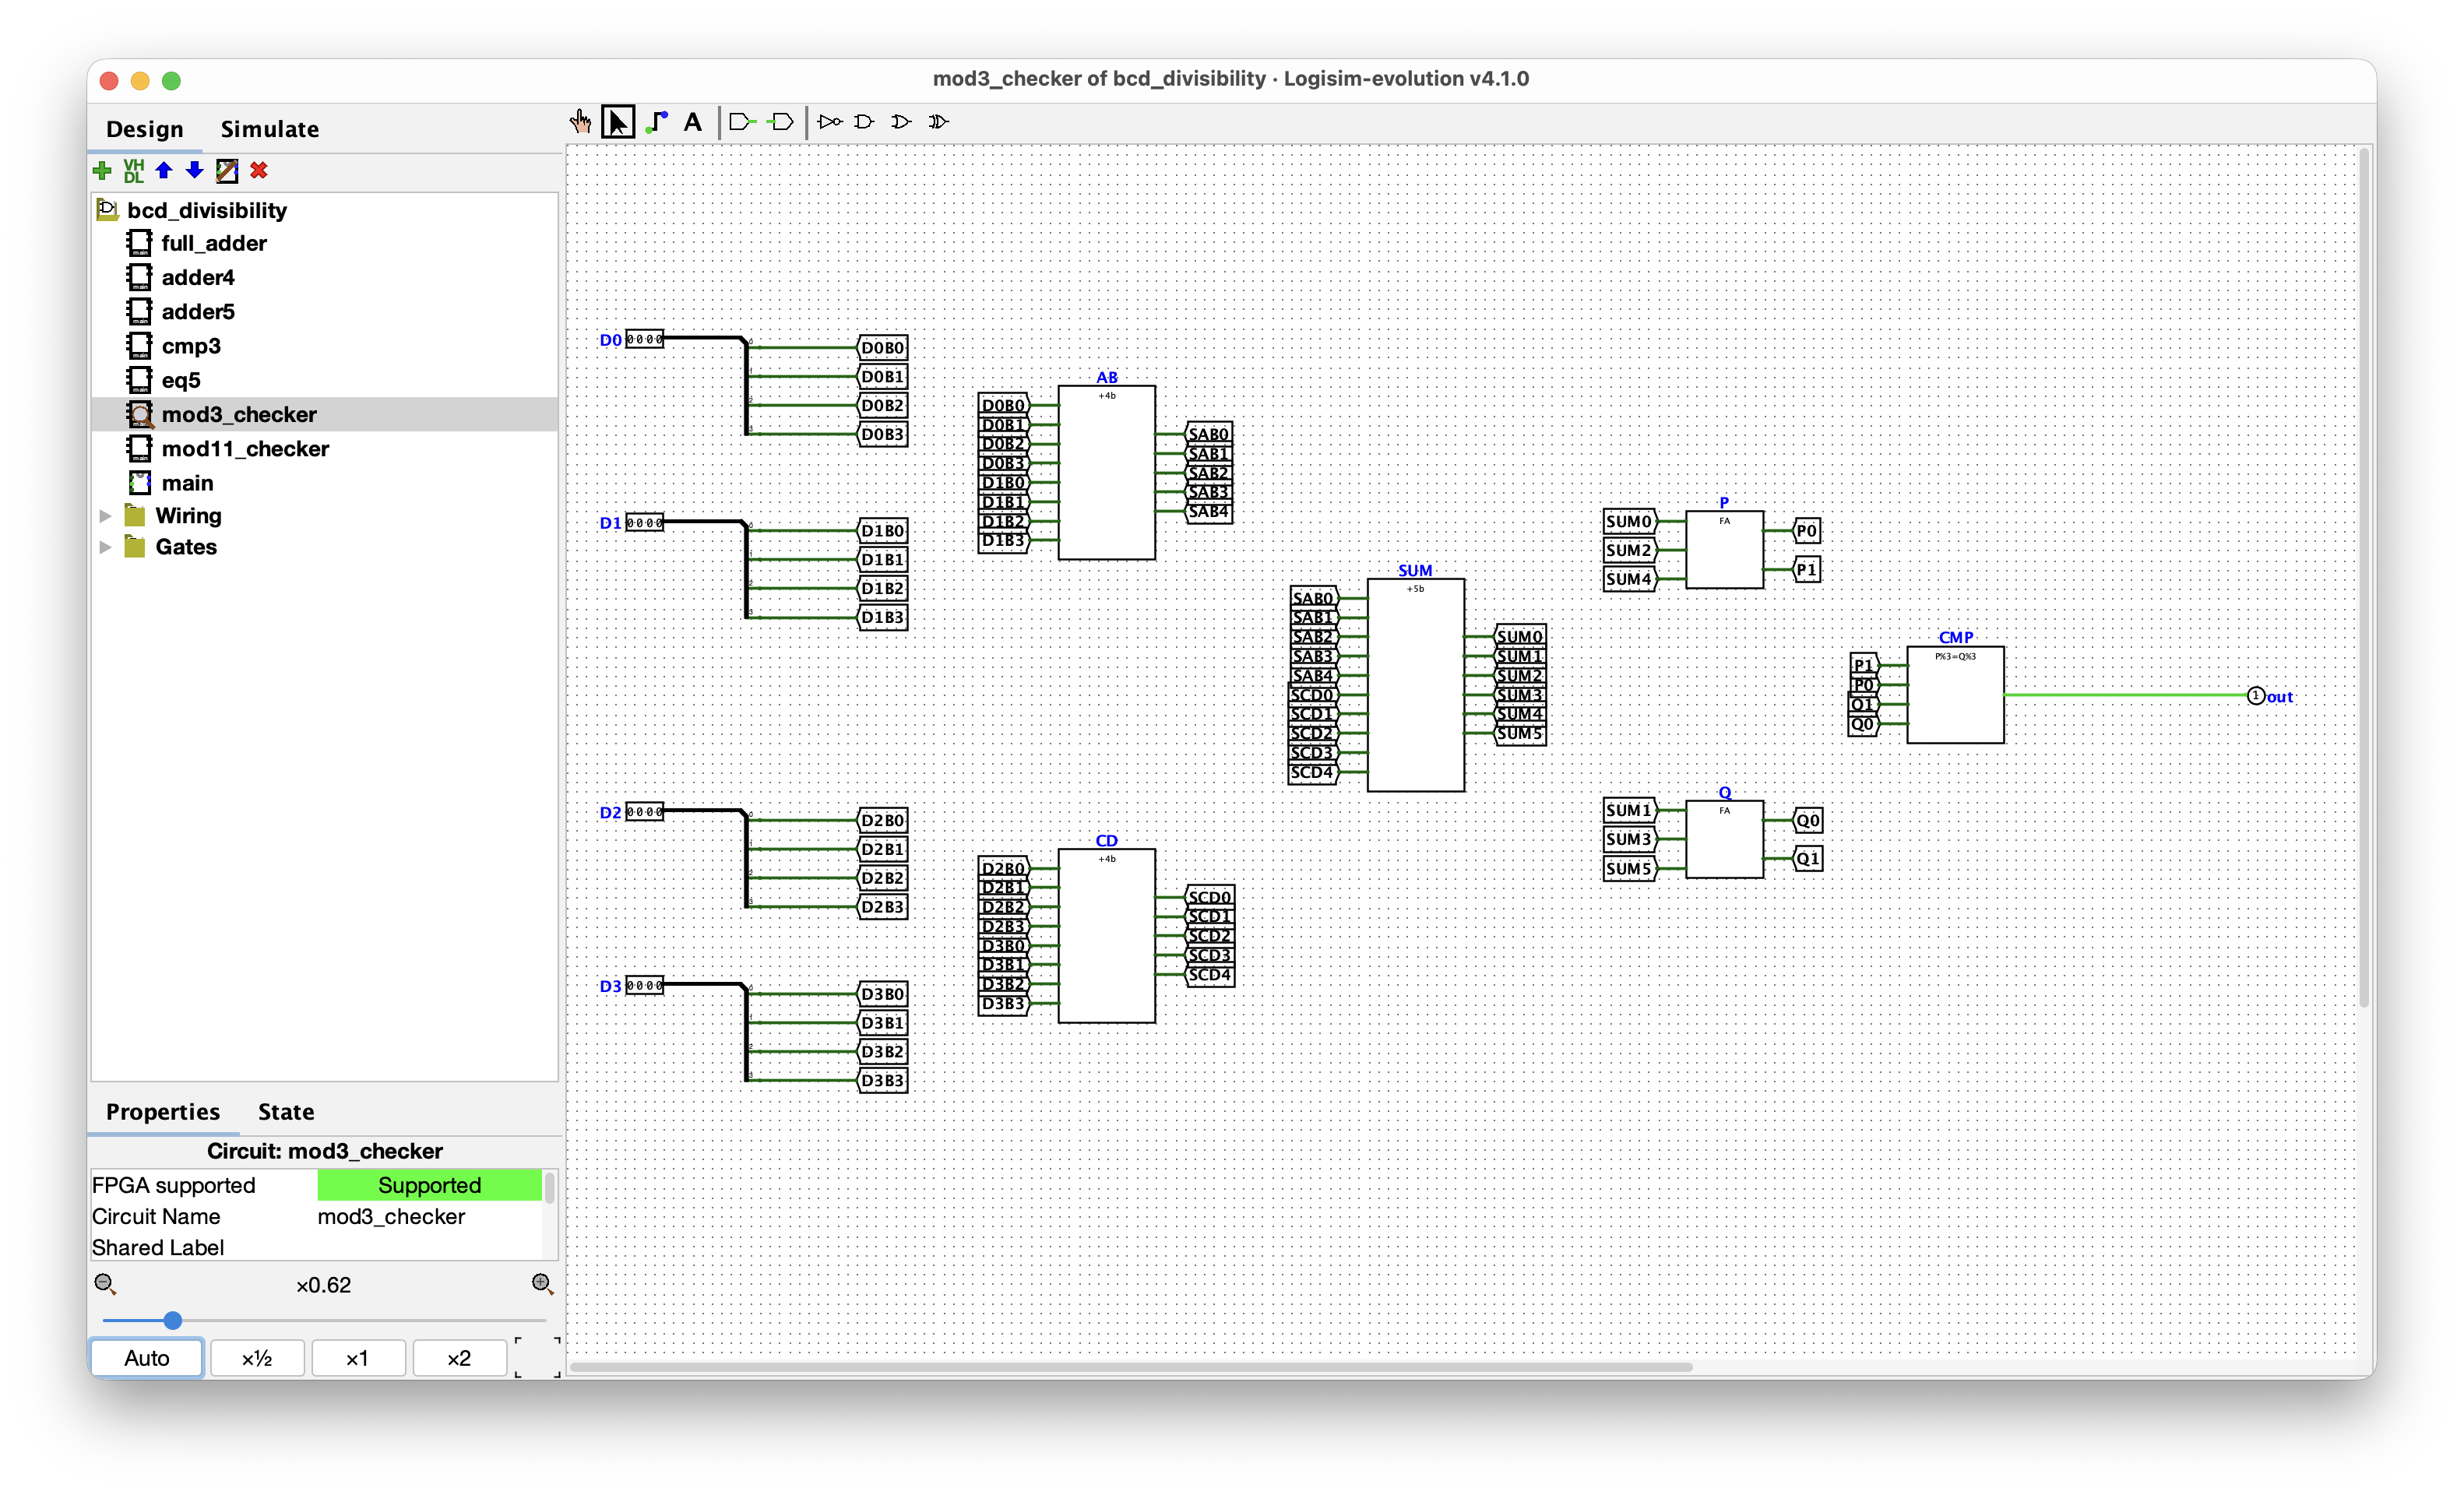
\includegraphics[width=0.95\textwidth]{figs/mod3-checker.png}
\end{center}

$D_0,D_1$ با \lr{adder4} جمع می‌شوند و $D_2,D_3$ نیز جدا؛ دو مجموع ۵بیتی با \lr{adder5} به مجموع کل $S=D_0{+}D_1{+}D_2{+}D_3$ (۶ بیت) تبدیل می‌شوند. سپس بیت‌های زوج $S$ با یک \lr{full\_adder} جمع می‌شوند ($\to P$) و بیت‌های فرد با یکی دیگر ($\to Q$)، و \lr{cmp3} شرط $P \bmod 3 {=} Q \bmod 3$ را چک می‌کند. 

\subsubsection*{معماری \lr{mod11\_checker}}

\begin{center}
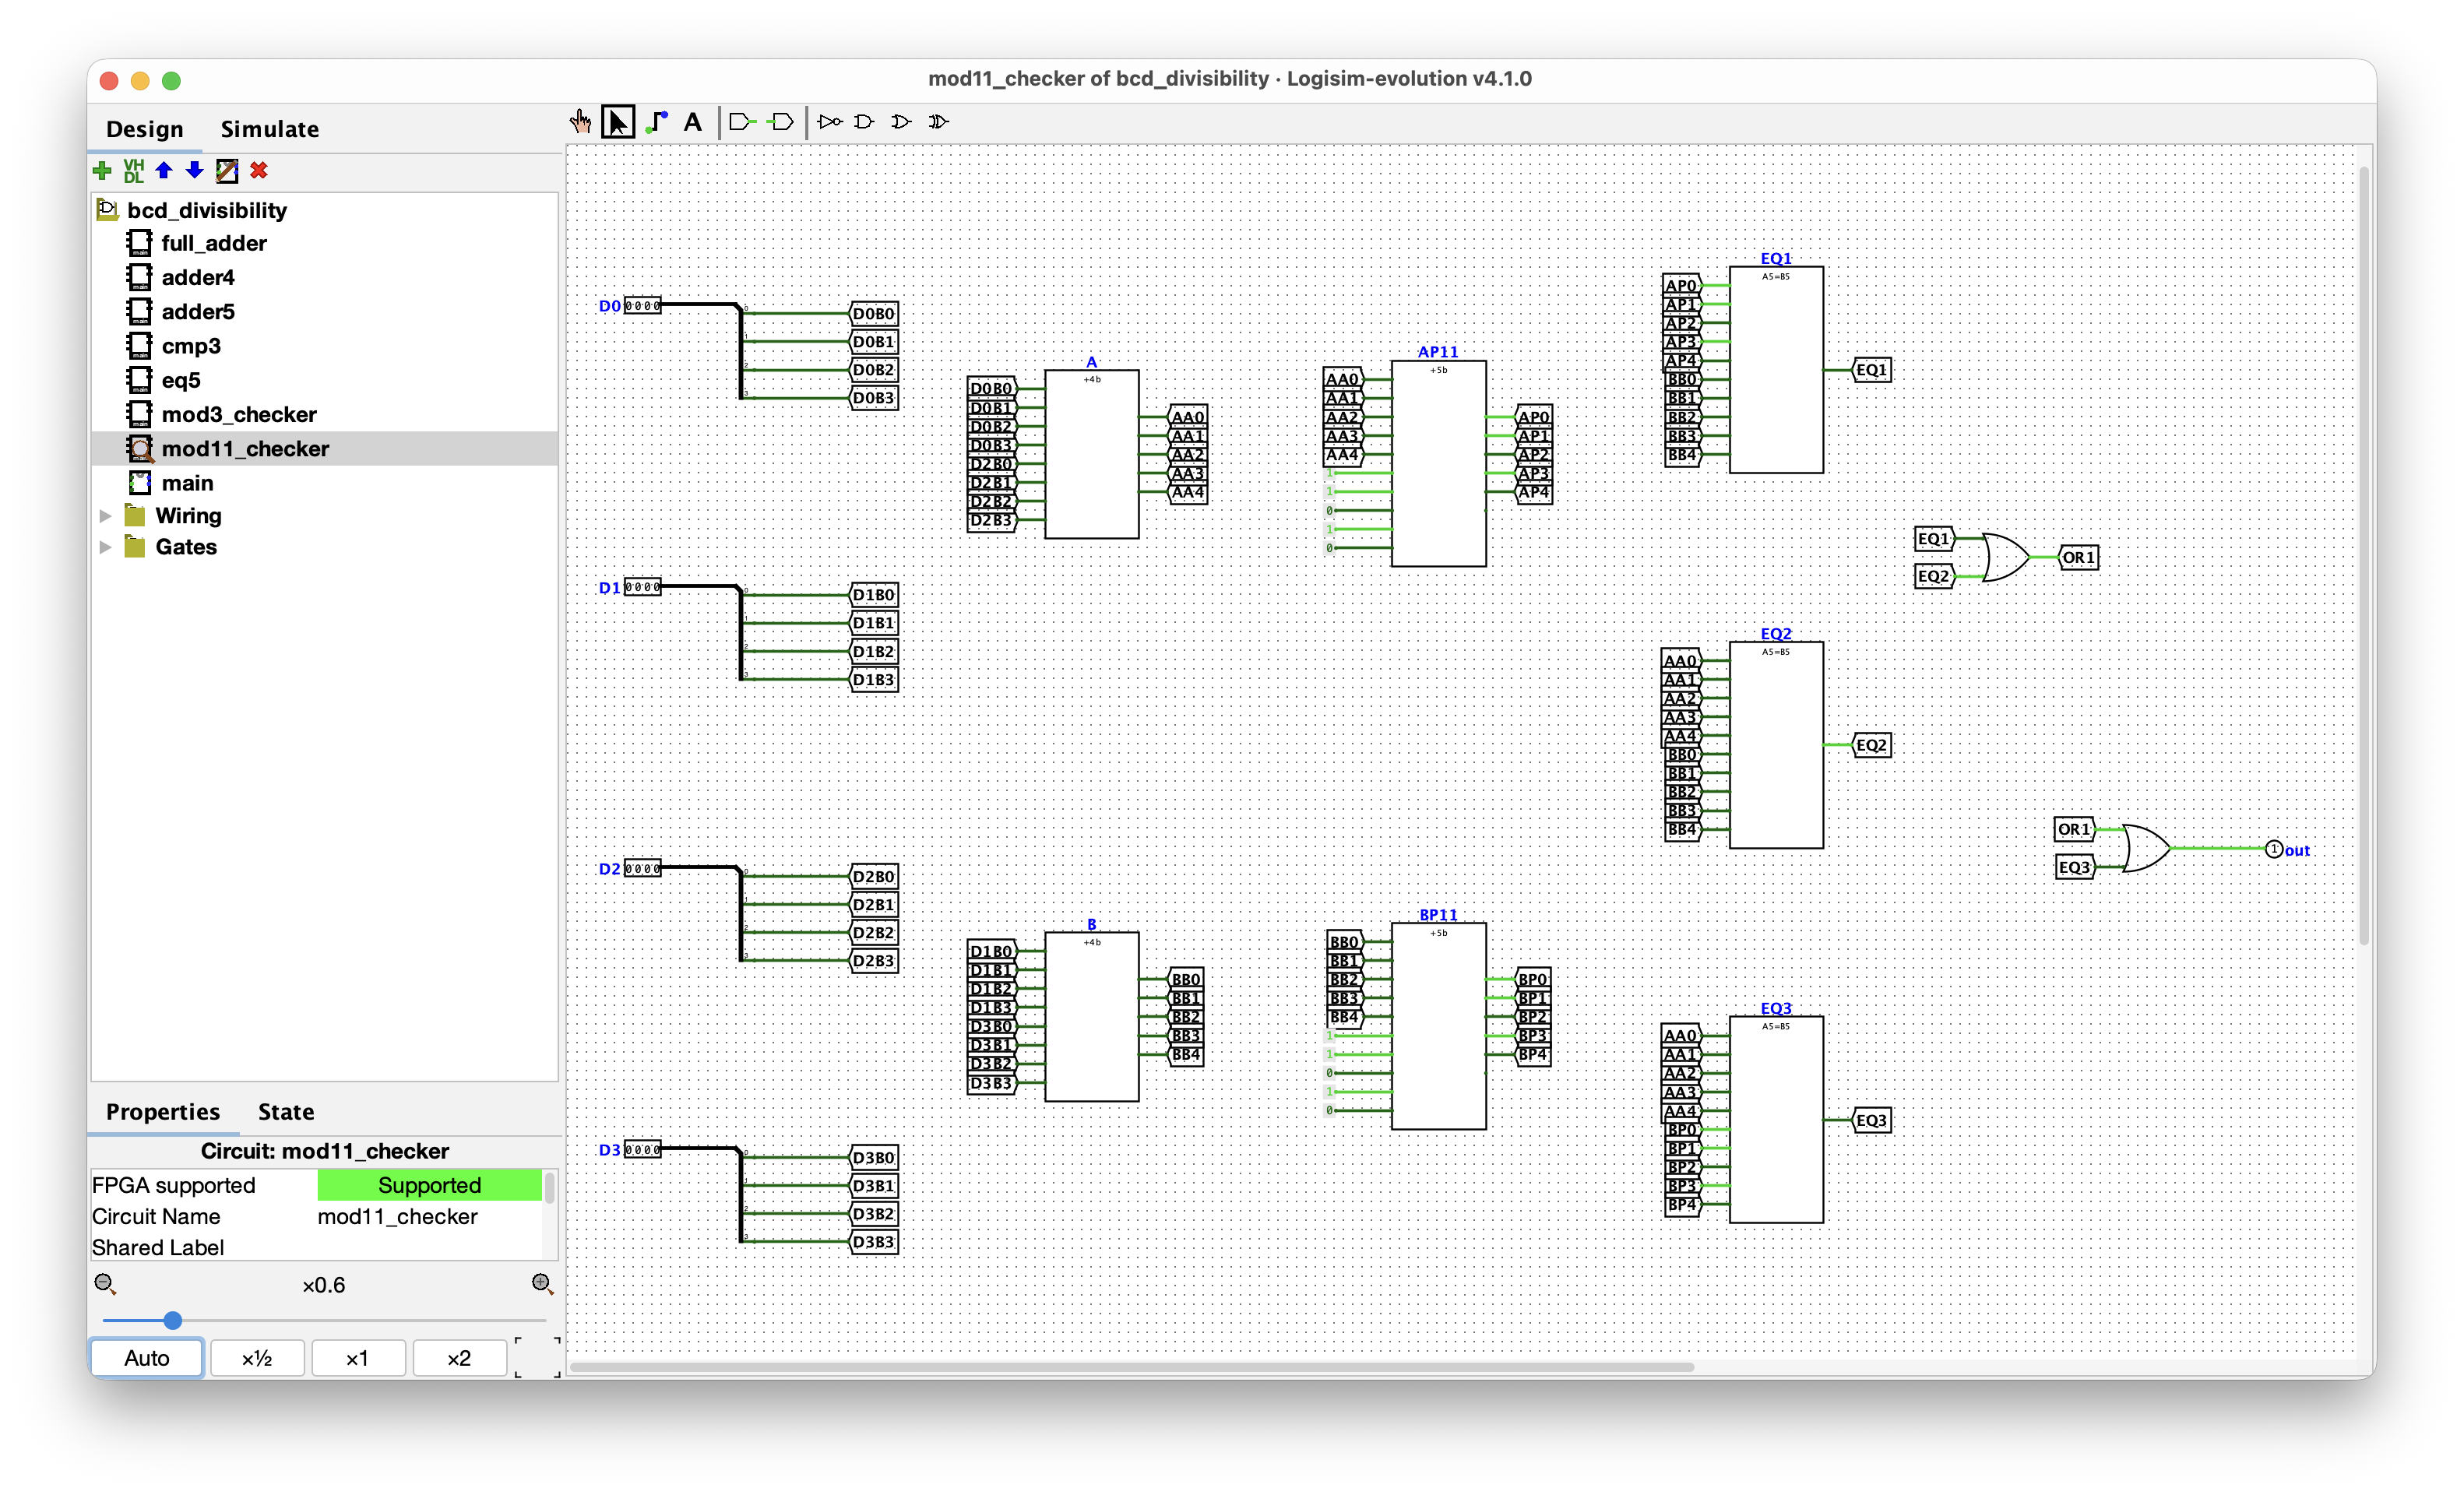
\includegraphics[width=0.95\textwidth]{figs/mod11-checker.png}
\end{center}

$A{=}D_0{+}D_2$ و $B{=}D_1{+}D_3$ با دو \lr{adder4} حساب می‌شوند؛ عدد ثابت ۱۱ ($=01011_2$) با ۵ قطعه‌ی \lr{Constant} تک‌بیتی مستقیما به ورودی $B$ هر \lr{adder5} وصل است تا $A{+}11$ و $B{+}11$ به‌دست بیایند. سه \lr{eq5} تساوی‌های $AP11{=}B$، $A{=}B$ و $A{=}BP11$ را چک می‌کنند و دو گیت \lr{OR} نهایی، خروجی سه مقایسه را \lr{OR} می‌کنند. 

\pagebreak

\subsubsection*{مدار \lr{main}}

برای مشاهده‌ی هم‌زمان هر دو خروجی، مدار \lr{main} دو بلوک \lr{mod3\_checker} و \lr{mod11\_checker} را روی همان ۴ پایه‌ی ورودی مشترک $D_0..D_3$ سوار می‌کند و دو خروجی \lr{mult\_of\_3} و \lr{mult\_of\_11} را جدا بیرون می‌دهد:

\begin{center}

\includegraphics[width=0.95\textwidth]{figs/main.png}
\end{center}

\pagebreak
\subsubsection*{نتایج تست}

هر ۸ مدار با بردار تست و از طریق خط فرمان \lr{Logisim} در حالت \lr{headless} (\lr{--test-vector}) تست شدند. \lr{full\_adder}, \lr{adder4}, \lr{adder5}, \lr{cmp3}, \lr{eq5} روی \emph{تمام} فضای ورودی‌شان تست شدند، و \lr{mod3\_checker}/\lr{mod11\_checker} روی {هر ۱۰۰۰۰ مقدار \lr{BCD} ممکن} ($0000$ تا $9999$).


خروجی واقعی اجرای \lr{run\_tests.sh}:

\begin{latin}
\lstinputlisting[basicstyle=\ttfamily\scriptsize]{figs/test_run_output.txt}
\end{latin}

چون هر دو مدار اصلی روی \emph{تمام} فضای ورودی معتبر تست شده‌اند، درستی مدار برای هر عدد \lr{BCD} چهاررقمی تضمین‌شده است.

\end{document}
